\documentclass[xcolor=pdftex,dvipsnames,table,mathserif,aspectratio=169]{beamer}
\usetheme{default}
\usetheme{metropolis}
%\usepackage{minted}
\usepackage{mathtools}
\usepackage{booktabs}
\usepackage{dcolumn}

\setbeamersize{text margin left=.3in,text margin right=.3in} 

\DeclarePairedDelimiter\abs{\lvert}{\rvert}%
\DeclarePairedDelimiter\norm{\lVert}{\rVert}%


%\usetheme{Darmstadt}
%\usepackage{times}
%\usefonttheme{structurebold}

\usepackage[english]{babel}
%\usepackage[table]{xcolor}
\usepackage{pgf,pgfarrows,pgfnodes,pgfautomata,pgfheaps}
\usepackage{amsmath,amssymb,setspace,centernot}
\usepackage[latin1]{inputenc}
\usepackage[T1]{fontenc}
\usepackage{relsize}
\usepackage{pdfpages}
\usepackage[absolute,overlay]{textpos} 


\newenvironment{reference}[2]{% 
  \begin{textblock*}{\textwidth}(#1,#2) 
      \footnotesize\it\bgroup\color{red!50!black}}{\egroup\end{textblock*}} 

\DeclareMathSizes{10}{10}{6}{6} 

\begin{document}
\title{Program Evaluation (c)- Propensity Scores}
\author{Chris Conlon}
\institute{Applied Econometrics}
\date{\today}

\frame{\titlepage}


\begin{frame}
\frametitle{Matching}
\begin{itemize}
\item Compare treated individuals to un-treated individuals with identical observable characteristics $X_i$.
\item Key assumption: everything about $Y_i(1) - Y_i(0)$ is captured in $X_i$; or $u_i$ is randomly assigned conditional on $X_i$.
\item Basic idea: The treatment group and the control group don't have the same distribution of observed characteristics as one another. 
\item \alert{Re-weight} the un-treated population so that it resembles the treated population.
\item Once distribution of $X_i$ is the same for both groups $ X_i | T_i \sim X_i$ then we assume all other differences are irrelevant and can just compare means.
\item Matching assumes \alert{all selection is on observables}.
\end{itemize}
\end{frame}



\begin{frame}
\frametitle{Why does any of this work?}
\small
Let  $F^{1}(x)$ be the distribution of characteristics in the treatment group, we can define the ATT as 
\begin{eqnarray*}
&&\mathbb{E}[Y(1) - Y(0) | T =1] =\mathbb{E}_{F^1(x)} \left[\mathbb{E}(Y(1) -Y(0) | T=1,X) \right] \\
&=&  \mathbb{E}_{F^1(x)} [\mathbb{E}(Y(1) | T=1,X)] -  \mathbb{E}_{F^1(x)} [\mathbb{E}(Y(0) | T=1,X)] \mbox{ linearity } 
\end{eqnarray*}
The first part we observe directly:
\begin{eqnarray*}
&=&  \mathbb{E}_{F^1(x)} [\mathbb{E}(Y(1) | T=1,X)] 
\end{eqnarray*}
But the counterfactual mean is not observed!
\begin{eqnarray*}
&=&  \mathbb{E}_{F^1(x)} [\mathbb{E}(Y(0) | T=1,X)] 
\end{eqnarray*}
But conditional independence does this for us:
\begin{eqnarray*}
 \mathbb{E}_{F^1(x)} [\mathbb{E}(Y(0) | T=1,X)]  =  \mathbb{E}_{F^1(x)} [\mathbb{E}(Y(0) | T=0,X)] 
\end{eqnarray*}
\end{frame}



\begin{frame}
\frametitle{Matching in Practice: \alert{Inverse Probability Weighting}}
How do we actually do this?
\begin{itemize}
\item Calculate a smoothed estimate of the treatment probability $\pi(x) = Pr(T_i =1 | x)$.
\begin{align*}
\frac{1}{n}\sum_{t \in \text{Treatment}} \frac{y_t}{\pi(x_t)} - \frac{1}{n} \sum_{s \in \text{Control}} \frac{y_s}{1-\pi(x_s)}
\end{align*}
\item How to get $\pi(x)$? Run a logit or probit.
\item We can stabilize the weights replace $w(x) =\frac{1}{\pi(x)}$ with:
\begin{align*}
w(x)=\frac{Pr(T=1)}{\pi(x)}  \mbox{ for } T_i=1 \quad
w(x)=\frac{Pr(T=0)}{1-\pi(x)} \mbox{ for } T_i=0
\end{align*}
\item This sometimes helps crazy big weights when treated group is small.
\end{itemize}
\end{frame}


\begin{frame}
\frametitle{Higher Dimensions}
So matching works great in dimension 1. But what if $dim(X) > 1$?
\begin{itemize}
\item True high-dimensional matching may be infeasible. There may be no set of weights such that:
$f(X_i | T_i=1) \equiv \int w_i f(X_i | T_i=0) \partial w_i $.
\item One solution is the nearest-neighbor approach in Abadie Imbens (2006).
\item This is still cursed in that our nearest neighbors get further away as the dimension grows.
\item Suppose instead we had a \alert{sufficient statistic}
\end{itemize}
\end{frame}

\begin{frame}
\frametitle{Propensity Score}
\begin{itemize}
\item Rosenbaum and Rubin propose the \alert{propensity score}
\begin{eqnarray*}
P(T_i  = 1 | X_i) \equiv P(X_i)
\end{eqnarray*}
\item They prove that the propensity score and any function of $X$, $b(X)$ which is finer serves as a \alert{balancing score}.
\item Finer implies that:
\begin{eqnarray*}
b(X^1) = b(X^2) &\implies& P(X^1) = P(X^2)\\
P(X^1) = P(X^2) & \centernot \implies & b(X^1) = b(X^2)
\end{eqnarray*}
\end{itemize}
\end{frame}


\begin{frame}
\frametitle{Propensity Score}
\begin{itemize}
\item Main result: If treatment assignment is strongly ignorable conditional on $X$ (CIA) then it is strongly ignorable $Y(1),Y(0) \perp T | X$ given any balancing score $b(X)$ including the propensity score:
\begin{align*}
Pr(T=1 | Y(1), Y(0),P(X))&= E[Pr(T=1| Y(1),Y(0),X) | P(X)] \\
&= E[Pr(T=1 | x) | P(X) ] = P(X)
\end{align*}
\item Also we require that $0 < P(X) < 1$ at each $X$ which is known as the \alert{support condition}.
\item The theorem implies that given $P(X)$ we have as if random assignment.
\end{itemize}
\end{frame}

\begin{frame}
\frametitle{Propensity Score}
\begin{itemize}
\item Instead of matching on $K$ dimensional $X$ we can now match on a one-dimensional propensity score
\item Thus the propensity score provides \alert{dimension reduction}
\item We still have to estimate the propensity score which is a high dimensional problem without \textit{ad-hoc} parametric restrictions.
\item Let us begin by assuming a can-opener.
\item An easy way would be to use $\pi(x)$ from logit or probit.
\end{itemize}
\end{frame}


\begin{frame}
\frametitle{Propensity Score}
Just like in the matching case the problem arises because we do not observe the counterfactual mean:
\begin{eqnarray*}
 E_{F^1(x)} [E(Y(0) | T=1,X)] 
\end{eqnarray*}
With conditional independence and the propensity score:
\begin{eqnarray*}
 E_{F^1(x)} [E(Y(0) | T=1,X)]  &=&  E_{F^1(x)} [E(Y(0) | T=0,X)] \\
 &=&  E_{F^1(x)} [E(Y(0) | T=0,P(X))] 
\end{eqnarray*}
\end{frame}

\begin{frame}
\frametitle{Kernel Matching}
How do we implement?
\begin{itemize}
\item Kernels are an obvious choice
\begin{eqnarray*}
\widehat{ATT} = \frac{1}{N_1} \sum_{i \in T=1} \left[Y_i - \frac{\sum_{j \in T=0} Y_j K\left(P(X_i) - P(X_j) \right) }{\sum_{s \in T=0}  K\left(P(X_i) - P(X_s) \right)}   \right]
\end{eqnarray*}
 where $N_1$ is the sample size of the treatment group \\
 and $K(u)$ is a valid Kernel weight (people tend to use Gaussian Kernels here)
\item As your propensity score gets further away from observation $i$ you get less weight
\item As $h \rightarrow 0$  (or $\sigma_h$) the window gets smaller and we use fewer neighbors.
\end{itemize}
\end{frame}


\begin{frame}
\frametitle{Kernel Matching}
\begin{itemize}
\item The usual caveats apply: $h$ determines the \alert{bias-variance} tradeoff
\item Choice of Kernel effects finite-sample properties
\item Here the \alert{common support} is important. We can only learn about cases where $P(X) \neq 1$ and $P(X) \neq 0$. If you always get treated (or not-treated) we cannot learn from this observation.
\item We also have to be careful in choosing $X$ so as not to violate CIA (too many $X$'s , too few $X$'s) $\rightarrow$ have to think carefully!
\item If you use propensity scores you will need a slide convincing us you have thought about why CIA holds for you!
\end{itemize}
\end{frame}



\begin{frame}
\frametitle{Gotcha!}
\small
Under CIA we know
\begin{eqnarray*}
G(Y(1),Y(0) | X, T) = G(Y(1),Y(0) | X)
\end{eqnarray*}
Suppose we add in $Z$, then we require that:
\begin{eqnarray*}
G(Y(1),Y(0) | X, Z, T) = G(Y(1),Y(0) | X, Z)
\end{eqnarray*}
\begin{eqnarray*}
G(Y(1),Y(0) | X, T) = \int G(Y(1),Y(0) | X, Z, T) dF(Z | X,T) \\
= G(Y(1),Y(0) | X)
\end{eqnarray*}
where the last part follows by CIA.
\begin{itemize}
\item Thus each element can depend on $T$ conditional on $Z,X$ but the average may not.
\item Mindless applications of matching can give you biased results!
\end{itemize}
\end{frame}


\begin{frame}
\frametitle{Matching and OLS}
\begin{itemize}
\item Recall that OLS is a special case of Kernel regression (and hence matching!)
\item Think about
\begin{eqnarray*}
Y  = \alpha + \beta T_i + u
\end{eqnarray*}
\item Assume that $E(u | T,X) = E(u | X)$ which is a conditional mean independence assumption
\item The we can get $\beta$ consistently (but not other variables) by running the following:
\begin{eqnarray*}
Y = \alpha + \beta T_i + \gamma X + v
\end{eqnarray*}
\item Again we are in the homogenous treatment world
\end{itemize}
\end{frame}



\begin{frame}
\frametitle{A Matching Example}
Here is an example where I found that matching was helpful in my own work with Julie Mortimer:
\begin{itemize}
\item We ran a randomized experiment where we removed Snickers bars from around 60 vending machines in office buildings in downtown Chicago.
\item We have a few possible control groups:
\begin{enumerate}
\item Same vending machine in other weeks (captures heterogeneous tastes in the cross section)
\item Other vending machines in the same week (might capture aggregate shocks, ad campaigns, etc.)
\end{enumerate}
\item We went with \#1 as \#2 was not particularly helpful.
\end{itemize}
\end{frame}

\begin{frame}
\frametitle{A Matching Example}
Major problem was that there was a ton of heterogeneity in the overall level of (potential) weekly sales which we call $M_t$.
\begin{itemize}
\item Main source of heterogeneity is how many people are in the office that week, or how late they work.
\item Based on total sales our average over treatment weeks was in the 74th percentile of all weeks.
\item This was after removing a product, so we know sales should have gone down!
\item How do we fix this without running the experiment for an entire year!
\item Can't use shares instead of quantities. Why?
\end{itemize}
\end{frame}

\begin{frame}
\begin{center}
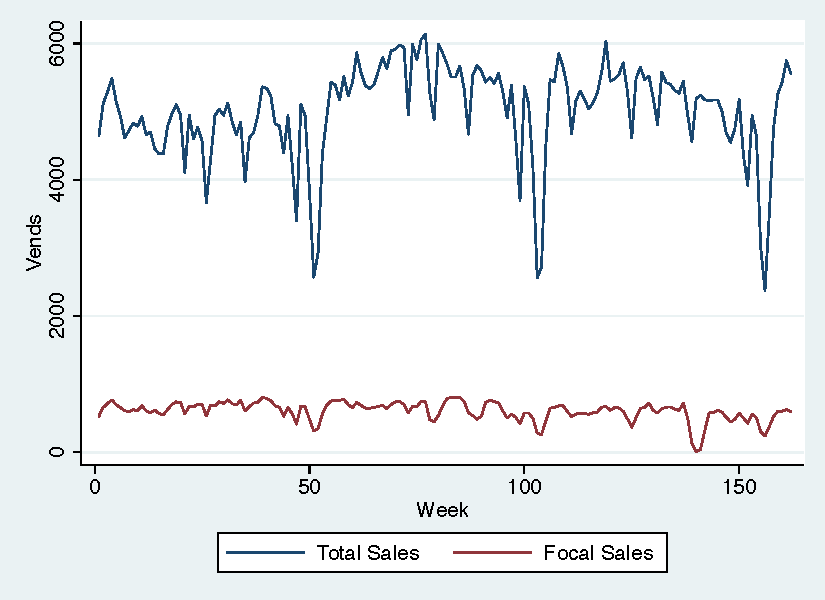
\includegraphics[width=4in]{./resources/figure1.pdf}
\end{center}
\end{frame}

\begin{frame}
\frametitle{A Matching Example}
Ideally we could just observe $M_t$ directly and use that as our matching variable $X$
\begin{itemize}
\item We didn't observe it directly and tried a few different measures:
\begin{itemize}
\item Sales at the soda machine next to the snack machine
\item Sales of salty snacks at the same machine (not substitutes for candy bars).
\item We used k-NN with $k=4$ to select control weeks -- notice we re-weight so that overall sales are approximately same (minus the removed product).
\end{itemize}
\item We also tried a more structured approach:
\begin{itemize}
\item Define controls weeks as valid IFF
\item Overall sales were weakly lower
\item Overall sales were not less than Overall Sales less expected sales less Snickers Sales.
\end{itemize}
\end{itemize}
\end{frame}


\begin{frame}
\begin{table}
\begin{center}
\tiny
\label{tab:nonparam}
\begin{tabular}{|l|rrrcrrcr|}
\hline
 & Control  & Control & Treatment& \hspace{-0.3in}& Treatment & Mean & \hspace{-0.3in} & \\
Product & Mean &  \%ile & Mean& \hspace{-0.3in} & \%ile &  Difference & \hspace{-0.3in}& \% $\Delta$\\
\hline \hline
\multicolumn{9}{|l|}{\emph{Vends}} \\ \hline
Peanut M\&Ms&359.9&73.6&478.3&\hspace{-0.3in}*&99.4&118.4& \hspace{-0.3in}*&32.9\\
Twix Caramel&187.6&55.3&297.1&\hspace{-0.3in}*&100.0&109.5& \hspace{-0.3in}*&58.4\\
Assorted Chocolate&334.8&66.7&398.0&\hspace{-0.3in}*&95.0&63.2& \hspace{-0.3in}*&18.9\\
Assorted Energy&571.9&63.5&616.2& \hspace{-0.3in}&76.7&44.3 & \hspace{-0.3in} &7.8\\
Zoo Animal Cracker&209.1&78.6&243.7&\hspace{-0.3in}*&98.1&34.6& \hspace{-0.3in}*&16.5\\
Salted Peanuts&187.9&70.4&216.3&\hspace{-0.3in}*&93.7&28.4 & \hspace{-0.3in} &15.1\\
Choc Chip Famous Amos&171.6&71.7&193.1&\hspace{-0.3in}*&95.0&21.5& \hspace{-0.3in}*&12.5\\
Ruger Vanilla Wafer&107.3&59.7&127.9& \hspace{-0.3in}&78.6&20.6& \hspace{-0.3in}*&19.1\\
Assorted Candy&215.8&43.4&229.6& \hspace{-0.3in}&60.4&13.7& \hspace{-0.3in}&6.4\\
Assorted Potato Chips&279.6&64.2&292.4&\hspace{-0.3in}*&66.7&12.8& \hspace{-0.3in}&4.6\\
Assorted Pretzels&548.3&87.4&557.7&\hspace{-0.3in}*&88.7&9.4& \hspace{-0.3in}&1.7\\
Raisinets&133.3&66.0&139.4& \hspace{-0.3in}&74.2&6.1& \hspace{-0.3in}&4.6\\
Cheetos&262.2&60.1&260.5& \hspace{-0.3in}&58.2&-1.8& \hspace{-0.3in}&-0.7\\
Grandmas Choc Chip&77.9&51.3&72.5& \hspace{-0.3in}&37.8&-5.4& \hspace{-0.3in}&-7.0\\
Doritos&215.4&54.1&203.1& \hspace{-0.3in}&39.6&-12.3& \hspace{-0.3in}*&-5.7\\
Assorted Cookie&180.3&61.0&162.4& \hspace{-0.3in}&48.4&-17.9& \hspace{-0.3in}&-10.0\\
Skittles&100.1&62.9&75.1&\hspace{-0.3in}*&30.2&-25.1& \hspace{-0.3in}*&-25.0\\
Assorted Salty Snack&1382.8&56.0&1276.2&\hspace{-0.3in}*&23.3&-106.7& \hspace{-0.3in}*&-7.7\\
Snickers&323.4&50.3&2.0&\hspace{-0.3in}*&1.3&-321.4& \hspace{-0.3in}*&-99.4\\ \hline
Total&5849.6&74.2&5841.3& \hspace{-0.3in}&73.0&-8.3& \hspace{-0.3in}&-0.1\\
\hline\end{tabular}
\end{center}
\tiny
Notes: Control weeks are selected through the-neighbor matching using four control observations for each treatment week.  Percentiles are relative to the full distribution of control weeks.
\end{table}
\end{frame}



\begin{frame}
\frametitle{Exercises}
\begin{itemize}
\item This would be a good time to work through the vignette for \texttt{cobalt}
 \url{https://cran.r-project.org/web/packages/cobalt/vignettes/cobalt_A0_basic_use.html}
 \item Compare the ATE for the Lalonde data with the IPW, Nearest Neighbor, and Propensity Score estimates.
 \item Then start the homework
\end{itemize}
\end{frame}




\end{document}
